\begin{figure}
\figuretitle{Figure~\ref{fig:intra_dimer_interface}}
\begin{fullpanelvar}
\begin{emptypanel}{}
    \node(dimer)[inner sep=0pt,below right]{\includegraphics[width=\linewidth,height=2in,keepaspectratio]{../results/dimer_interface/output/dimer_interface_overview_cropped.png}};
    %
    \node(captionA)[inner sep=0pt,above left] at (dimer.north west) {\normalsize\textbf{\figurepanela}};
    %
    \path (dimer.south west)++(1.75,1.45) coordinate (roi_left_SW); 
    \path (dimer.south west)++(2.5,2.45) coordinate (roi_left_NE);
    \node(dimer_roi_left) [fit={(roi_left_SW) (roi_left_NE)}, dashedrectanglefit] {};    
    %
    %
    \path (dimer.south)++(-0.25,1.75) coordinate (roi_center_SW); 
    \path (dimer.south)++(0.25,2.25) coordinate (roi_center_NE);
    \node(dimer_roi_center) [fit={(roi_center_SW) (roi_center_NE)}, dashedrectanglefit] {};    
    %
    %
    \node(closeup_143)[inner sep=0pt,right=1cm of dimer]{\includegraphics[width=\linewidth,height=2in,keepaspectratio]{../results/dimer_interface/output/dimer_interface_E143_closeup_yb_cropped.png}};
    %
    \node(closeup_143_rect) [fit=(closeup_143), dashedrectanglefit] {};
    %
    \node(D140_E143_E147_ROI_label) [above, inner sep=5pt, align=center] at (closeup_143.north) {D140/E143/E147 Intra-Dimer Region};
    %
    % D140
    \path (closeup_143.north)++(1.5,-0.4)  coordinate (cD140);
    \node(D140) [above, inner sep=0pt, font=\small, font=\bfseries] at (cD140) {D140};
    % E143
    \path (closeup_143.north)++(-2.25,-1)  coordinate (cE143);
    \node(E143) [above, inner sep=0pt, font=\small, font=\bfseries] at (cE143) {E143};
    % E275
    \path (closeup_143.east)++(-1,0)  coordinate (cE275);
    \node(E275) [above, inner sep=0pt, font=\small, font=\bfseries] at (cE275) {E275};
    % E147
    \path (closeup_143.west)++(0.75,-0.75)  coordinate (cE147);
    \node(E147) [above, inner sep=0pt, font=\small, font=\bfseries] at (cE147) {E147};
    % D278
    \path (closeup_143.east)++(-1.75,-1)  coordinate (cD278);
    \node(D278) [above, inner sep=0pt, font=\small, font=\bfseries] at (cD278) {D278};
    % D280
    \path (closeup_143.south)++(1,0.35)  coordinate (cD280);
    \node(D280) [above, inner sep=0pt, font=\small, font=\bfseries] at (cD280) {D280};
    %
    %
    %
    \node(closeup_310)[inner sep=0pt,below=1cm of dimer]{\includegraphics[width=\linewidth,height=2in,keepaspectratio]{../results/dimer_interface/output/dimer_interface_D310_closeup_yb_cropped.png}};
    %
    \node(closeup_310_rect) [fit=(closeup_310), dashedrectanglefit] {};
    %
    \node(D310_ROI_label) [above, inner sep=5pt, align=center] at (closeup_310.north) {D310 Intra-Dimer Region};
    % D310
    \path (closeup_310.north)++(0,-0.5)  coordinate (cD310);
    \node(D310) [above, inner sep=0pt, font=\small, font=\bfseries] at (cD310) {D310};
    % R251_L
    \path (closeup_310.west)++(0.5,-1)  coordinate (cR251_L);
    \node(R251_L) [above, inner sep=0pt, font=\small, font=\bfseries] at (cR251_L) {R251};
    % R251_R
    \path (closeup_310.east)++(-0.5,-1)  coordinate (cR251_R);
    \node(R251_R) [above, inner sep=0pt, font=\small, font=\bfseries] at (cR251_R) {R251};
    % K276
    \path (closeup_310.south)++(0,0.25)  coordinate (cK276);
    \node(K276) [above, inner sep=0pt, font=\small, font=\bfseries] at (cK276) {K276};
    %    
    \node(dimerdeonative)[inner sep=0pt,right=2cm of closeup_310_rect.north east,anchor=north]{\includegraphics[width=\linewidth,height=0.75in,keepaspectratio]{../results/dimer_interface/output/dimer_deo_native_bsa_cropped.png}};
    %
    \path (dimerdeonative.south west)++(0,-0.25cm) coordinate (dimer_dim_left); 
    \path (dimerdeonative.south)++(-0.4cm,-0.25cm) coordinate (dimer_dim_center_left); 
    \path (dimerdeonative.south)++(0.4cm,-0.25cm) coordinate (dimer_dim_center_right); 
    \path (dimerdeonative.south east)++(0,-0.25cm) coordinate (dimer_dim_right); 
    \draw[-] (dimer_dim_left) -- (dimer_dim_center_left);
    \draw[-] (dimer_dim_center_right) -- (dimer_dim_right);
    \draw[-] (dimer_dim_left)++(0,0.1cm) -- (dimer_dim_left)++(0,-0.1cm);
    \draw[-] (dimer_dim_right)++(0,0.1cm) -- (dimer_dim_right)++(0,-0.1cm);
    %
    \path (dimerdeonative.south)++(0,-0.5cm) coordinate (coord_dimer_deo_native_bsa_label); 
    \node(dimerdeonativebsalabel) [below, inner sep=2pt, align=center] at (coord_dimer_deo_native_bsa_label) {6OWV, 2536 \AA\textsuperscript{2} BSA};
    \node(dimer_deo_native_dim_label) [below, inner sep=3pt, align=center] at (dimerdeonative.south) {73 \AA};
    % 
    \node(dimer_1sji)[inner sep=0pt,below=0.5cm and 0.5cm of dimerdeonativebsalabel]{\includegraphics[width=\linewidth,height=0.75in,keepaspectratio]{../results/dimer_interface/output/dimer_1sji_bsa_cropped.png}};
    %
    \path (dimer_1sji.south west)++(0,-0.25cm) coordinate (dimer_1sji_dim_left); 
    \path (dimer_1sji.south)++(-0.4cm,-0.25cm) coordinate (dimer_1sji_dim_center_left); 
    \path (dimer_1sji.south)++(0.4cm,-0.25cm) coordinate (dimer_1sji_dim_center_right); 
    \path (dimer_1sji.south east)++(0,-0.25cm) coordinate (dimer_1sji_dim_right); 
    \draw[-] (dimer_1sji_dim_left) -- (dimer_1sji_dim_center_left);
    \draw[-] (dimer_1sji_dim_center_right) -- (dimer_1sji_dim_right);
    \draw[-] (dimer_1sji_dim_left)++(0,0.1cm) -- (dimer_1sji_dim_left)++(0,-0.1cm);
    \draw[-] (dimer_1sji_dim_right)++(0,0.1cm) -- (dimer_1sji_dim_right)++(0,-0.1cm);
    %
    \path (dimer_1sji.south)++(0,-0.5cm) coordinate (coord_dimer_1sji_bsa_label); 
    \node(1sji_bsa_label) [below, inner sep=2pt, align=center] at (coord_dimer_1sji_bsa_label) {1SJI, 1815 \AA\textsuperscript{2} BSA};
    \node(dimer_1sji_dim_label) [below, inner sep=3pt, align=center] at (dimer_1sji.south) {79 \AA};
    %
    \node(captionB)[inner sep=0pt,above left] at (dimerdeonative.north west) {\normalsize\textbf{\figurepanelb}};
    %
    \node(overlay_rmsd)[inner sep=0pt,right=3cm of dimerdeonative.north east, anchor=north]{\includegraphics[width=\linewidth,height=1.75in,keepaspectratio]{../results/dimer_interface/output/dimer_interface_overlay_1sji_rmsd_cropped.png}};
    %
    \node(overlay_rmsd_label) [below, inner sep=2pt, align=center] at (overlay_rmsd.south) {Gray: 1SJI Chain A\\Color: 6OWV Chain A};
    %
    \node(spectrumbarrmsd)[inner sep=0pt,below=0.5cm and 0.5cm of overlay_rmsd_label]{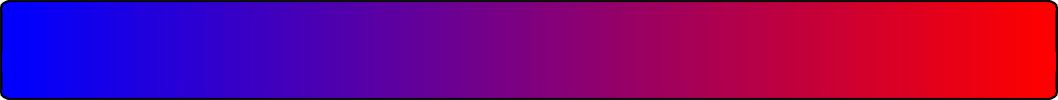
\includegraphics[width=\linewidth,height=0.05in,keepaspectratio]{../bin/colormaps/resource/pymol_blue_red_spectrum.png}};
    %
    \node(rmsdlabel) [above, inner sep=2pt] at (spectrumbarrmsd.north) {RMSD};
    %
    \node(rmsdlabelwest) [below, inner sep=6pt, align=center] at (spectrumbarrmsd.north west) {1.5 \AA};
    \node(rmsdlabeleast) [below, inner sep=6pt, align=center] at (spectrumbarrmsd.north east) {18 \AA};
    %
    \path (overlay_rmsd.north east)++(-0.25,-0.25) coordinate (arcstart);
    %
    \path[-] (dimer_roi_left.north) edge (closeup_143_rect.north west);
    \path[-] (dimer_roi_center.south) edge (closeup_310_rect.north east);
    \draw[<-, line width=0.2mm] (arcstart) arc (30:90:1);
    \node(arclabel) [below, inner sep=3pt] at (arcstart) {\ang{20}};
\end{emptypanel}
\end{fullpanelvar}
\caption[The intra-dimer interface of cardiac calsequestrin]{\textbf{\headingsubsubsectionfour}.\figurepanelcaptiona Dimer with ytterbium (Yb) sites (magenta spheres) within its interior cavity. Closeups focus on Yb positions that bridge dimer chains A and B: relatively strong coordination interactions are observed in a narrow intra-dimer cleft (right detail panel), while a site of weaker interaction and weaker occupancy is identified in the intra-dimer cavity (lower detail panel). \figurepanelcaptionb Comparison of a previously published cardiac calsequestrin dimer (1SJI) to the  more tightly-packed dimer that we report. The tightly-packed dimer results primarily from rigid body rotation of the dimer chains inward (for a single chain, we observe \ang{20} counter-clockwise rotation in the plane of the page when the other chain is fixed to the reference dimer). The inward rotation produces an increase in buried surface area (BSA) in thioredoxin domains II and III.}
\label{fig:intra_dimer_interface}
\end{figure}
